\chapter{Intégrale de Lebesgue}
\section{Principe général}
Les deux chapitres précédents ont montré comment il était possible de définir
une notion de "longueur" généralisée ainsi qu'une classe applications possédant
de bonnes propriétés vis à vis des images réciproques d'intervalles. Pour
clôturer le programme fixé en début du chapitre 1 et visant à introduire une
notion d'intégrale utilisant un découpage de l'ensemble d'arrivée, il reste à
assembler ces deux outils.
\section{Intégrale des applications positives}
Dans l'intégration au sens de Riemann, qui se base sur une subdivision de
l'intervalle de départ, les applications qui se traitent le plus naturellement
sont celles en escalier, pour lesquelles le calcul de l'aire sous-tendue à leur
graphe est immédiat. Dans le cadre Lebesgue, la subdivision portant sur
l'ensemble des valeurs, un travail préalable important a été nécessaire afin de
pouvoir calculer une mesure ("longueur" généralisée pour notre propos \dots).
Ici, les applications dont l'aire sous-tendue au graphe sera obtenue
immédiatement sont beaucoup plus générales: il suffit que l'ensemble des
\underline{valeurs} prises soit fini et que l'image réciproque du singleton
formé par l'une de ses valeurs soit mesurable. Ceci conduit à la définition
ci-dessous:
\begin{mandatory}
\begin{defn}\label{ch3:int1}
Soit $(E, \mathcal{T}, \mu)$ un espace mesuré.
Soit $f$ une application étagée (relativement à la tribu $\mathcal{T}$) positive s'écrivant~:
\[
f(x) = \sum_{i=1}^n a_i 1_{A_i}(x)
\]
avec $A_i, i=1 \dots n$ parties mesurables formant une partition de $E$.
L'intégrale de $f$ est par définition~:
\[
\int_E f d\mu = \sum_{i=1}^n a_i \mu(A_i)
\]
\end{defn}
\end{mandatory}
On notera que la sommation portant uniquement sur un nombre fini de termes
positifs il ne peut y avoir de
problème de définition ou de convergence (la valeur de l'intégrale peut
néanmoins être $+\infty$). La classe des fonctions étagées,
transposition au cadre de l'intégrale de Lebesgue de la classe des fonctions en escalier est beaucoup plus riche que cette dernière.

\begin{exercice}
\begin{itemize}
  \item Montrer que toute fonction en escalier est étagée.
  \item Soit $1_{\mathbb{Q}\cap [0,1]}$ l'application indicatrice de l'ensemble
  des rationnels dans l'intervalle $[0,1]$. Montrer qu'elle est étagée. Est-elle
  en escalier ?
  \item Calculer l'intégrale de l'application précédente en prenant pour mesure
  la mesure de Lebesgue.
\end{itemize}
\end{exercice}
\begin{rem}
La valeur de l'intégrale est indépendante de l'écriture de $f$. Soit
une autre partition $(B_i)_{i=1}^m$ formée de parties mesurables et 
telle que $f(x) = \sum_{i=1}^m b_i 1_{B_i}(x)$. On a nécessairement
$a_i = b_j$ si $A_i \cap B_j \neq \emptyset$, d'où par additivité de
$\mu$ sur des parties disjointes~:
\begin{multline*}
\sum_{i=1}^n a_i \mu(A_i) = \sum_{i=1}^n \sum_{j=1}^m a_i \mu(A_i \cap
B_j) = \\ \sum_{i=1}^n \sum_{j=1}^m b_j \mu(A_i \cap B_j)=  \sum_{j=1}^m b_j
\mu(B_j)
\end{multline*}
\end{rem}
\begin{mandatory}
\begin{prop}\label{int:1}
Soient $f,g$ deux applications étagées positives, et soit $\lambda> 0$. On a~:
\begin{align*}
&\int_E \left( \lambda f + g \right) d\mu = \lambda \int_E f d\mu + \int_E g d
\mu\\ &\mbox{ si } f \leq g , \quad \int_E f d\mu \leq \int_E g d \mu
\end{align*}
\end{prop}
\end{mandatory}
\begin{proof}
Soient les deux expressions de $f,g$~:
\[
f = \sum_{i=1}^n a_i 1_{A_i}, \quad g = \sum_{j=1}^m b_j 1_{B_j}
\]
avec $(A_i)$ et $(B_j)$ familles disjointes.
$\lambda f +g $ est étagée positive et a pour expression~:
\[
\lambda f + g = \sum_{i=1}^n \sum_{j=1}^m (\lambda a_i + b_j) 1_{A_i \cap
B_j}
\]
d'où~:
\begin{align*}
\int_E \left( \lambda f +g \right) d \mu & = \sum_{i=1}^n \sum_{j=1}^m (\lambda
a_i + b_j) \mu(A_i \cap B_j)\\ &  = \sum_{i=1}^n \sum_{j=1}^m \lambda a_i
\mu(A_i\cap B_j) + b_j \mu(A_i \cap B_j)\\ & = \sum_{i=1}^n a_i \mu(A_i) + \sum_{j=1}^m b_j \mu(B_j)\\
	& = \int_E \lambda f d \mu + \int_E g d\mu
\end{align*}
Pour la deuxième proposition, on écrit~:
\begin{align*}
&f = \sum_{i=1}^n \sum_{j=1}^m a_i 1_{A_i\cap B_j} \\
&g = \sum_{i=1}^n \sum_{j=1}^m b_j 1_{A_i\cap B_j}
\end{align*}
et on remarque que sur les ensembles  non vides de la forme $A_i\cap B_j$ on a
nécessairement $a_i \geq b_j$.
\end{proof}
\begin{mandatory}
\begin{prop}{(Changement de variable)}
Soient $(E, \mathcal{T}), (F, \mathcal{F})$ deux espaces mesurables. Soit $\phi
\colon E \to F$ une application mesurable. Soit $\mu$ une mesure sur $E$ et
$\phi_*\mu$ la mesure image de $\mu$. Pour toute application étagée positive $f
\colon F \to \mathbb{R}^+$, l'application $\tilde{f} = f \circ \phi$ est étagée
positive et l'on a:
\[
\int_F f d\phi_*\mu = \int_E \tilde{f} d \mu
\]
\end{prop}
\end{mandatory}
\begin{proof}
Soit $f = \sum_{i=1}^N a_i 1_{A_i}$ une écriture de $f$ avec $(A_i)_{i=1\dots
N}$ une partition de $F$ par des parties mesurables. La famille
$\left(\phi^{-1}(A_i)\right)_{i=1\dots N}$ est une partition de $E$ formée de
parties mesurables car $\phi$ est mesurable. On vérifie aisément que:
\[
\tilde{f} = \sum_{i=1}^N a_i 1_{\phi^{-1}(A_i)}
\] 
On a:
\begin{align*}
\int_E \tilde{f} d\mu & = \sum_{i=1}^N a_i \mu\left(\phi^{-1}(A_i)\right) \\
& = \sum_{i=1}^N a_i \phi^*\mu\left(A_i\right) = \int_F f d\phi_*\mu
\end{align*} 
\end{proof}
La proposition précédente ressemble à une relation d'adjonction entre
opérateurs. Pour toute application mesurable $f \colon F \to \mathbb{R}$, 
l'image réciproque de $f$ par $\phi$ est l'application mesurable $\tilde{f}$, 
que l'on note généralement $\phi^*f = f \circ \phi$. On définit ainsi un
opérateur sur les fonctions mesurables appelé image réciproque. Si l'on
interprète formellement l'intégrale comme un crochet de dualité, 
l'operateur $\phi^*$ agissant sur les fonctions mesurables et l'opérateur
$\phi_*$ agissant sur les mesures sont adjoints l'un de l'autre.
En posant:
\[
\langle \mu, g \rangle = \int d \mu
\]
on a ainsi:
\[
\langle f_*\mu, g \rangle = \langle \mu, f^*g \rangle
\]

Un cas important du changement de variable est obtenu en prenant un espace
mesurable $(E, \mathcal{T})$ et en se donnant $A \in \mathcal{T}$ une partie
mesurable. On munit $A$ de sa tribu induite $\mathcal{T}_A$, l'injection
canonique $i \colon A \hookrightarrow E$ est alors mesurable.
 Soit $\mu$ une mesure sur $E$ et $\mu_A$ la restriction de $\mu$ à $A$. 
 Soit $f = \sum_{i=1}^N a_i 1_{A_i}$ une application étagée positive sur $E$. La
 formule du changement de variable donne:
\[
\int_E f d(i_*\mu_A) = \int_A (f \circ i) d \mu_A
\]
Le premier terme a pour expression:
\begin{align*}
\int_E f d(i_*\mu_A) & = \sum_{i=1}^N a_i \mu_A\left(i^{-1}(A_i)\right)  \\
& =\sum_{i=1}^N a_i \mu_A\left(A_i \cap A \right) = \sum_{i=1}^N a_i \mu
\left(A_i \cap A \right)
\end{align*}
On a $1_{A\cap B} = 1_A . 1_B$ pour tout couple $(A,B)$ de parties de $E$. On
peut donc écrire:
\[
\sum_{i=1}^N a_i \mu
\left(A_i \cap A \right) = \int_E f . 1_A d\mu
\]
On a ainsi montré l'importante proposition:
\begin{mandatory}
\begin{prop}{(Intégrale sur une partie mesurable)}
Soit $f$ une application étagée positive sur $(E,\mathcal{T},\mu)$ et soit $A
\subset E$ une partie mesurable. On a:
\[
\int_A (f \circ i_A) d \mu_A = \int_E f . 1_A d\mu
\]
avec $i_A$ injection canonique de $A$ dans $E$.
\end{prop}
\end{mandatory}
La formule précédente conduit à la relation de Chasles. En effet, pour toute
partie mesurable $A$, son complémentaire $A^c$ est mesurable et de plus $1_E =
1_A + 1_{A^c}$, d'où pour toute application étagée positive $f$ sur $E$:
\[
\int_E f d \mu = \int_A (f \circ i_A) d \mu_A + \int_{A^c} (f \circ i_{A^c}) d
\mu_{A^c}
\]
On généralise immédiatement ceci à tout couple de parties mesurables disjointes:
\begin{mandatory}
\begin{prop}{(Formule de Chasles)}
Soit $f$ une application étagée positive sur $(E,\mathcal{T},\mu)$ et soit
$(A,B)$ un couple de parties mesurables disjointes. On a:
\[
\int_A (f \circ i_A) d \mu_A  + \int_B (f \circ i_B) d \mu_A= \int_{A\cup B} (f
\circ i_{A\cup B}) d\mu_{A\cup B}
\]
\end{prop}
\end{mandatory}
Afin d'alléger les notations, on supprime le plus souvent les injections
canoniques ainsi que les indices dans les mesures restreintes, la formule de
Chasles devient ainsi:
\[
\int_A f d \mu  + \int_B f d \mu= \int_{A\cup B} f d\mu
\]
qui est l'écriture la plus courante.
\begin{mandatory}
\begin{prop}
Soit $(f_n)_{n \in \mathbb{N}}$ une suite croissante d'applications
étagées positives, convergeant simplement vers une application étagée
positive $f$. On a~:
\[
\int_E f d\mu = \lim_{n\to +\infty} \int_E f_n d \mu
\]
\end{prop}
\end{mandatory}
\begin{proof}
Il est clair, au vu de la proposition précédente, que la suite $\int_E
f_n d \mu$ est croissante, bornée par $\int_E f d \mu$, donc
converge. Soit maintenant $\epsilon > 0$ et soit $f = \sum_{i=1}^N a_i
1_{A_i}$ une écriture de $f$. On pose~:
\[
A_i(n,\epsilon) = \{ x \in A_i | f_n(x) > (1-\epsilon)a_i \}, \quad
i=1\dots N
\]
et~:
\[
g_n = \sum_{i=1}^N (1-\epsilon)a_i 1_{A_i(n,\epsilon)}
\]
chaque $A_i(n,\epsilon)$ est mesurable car intersection du mesurable $A_i$
avec image réciproque de $](1-\epsilon)a_i, +\infty[$ par l'application
mesurable $f_n$. De plus, la suite $(A_i(n,\epsilon))_{n\in \mathbb{N}}$ est croissante au sens de
l'inclusion, de réunion $A_i$, d'où $\lim_{n\to+\infty}
\mu(A_i(n,\epsilon)) = \mu(A_i)$.
On a alors~:
\[
\int_E g_n d\mu = \sum_{i=1}^N (1-\epsilon)a_i \mu(A_i(n,\epsilon))
\leq \int_E f_n d \mu
\]
et~:
\[
\lim_{n\to+\infty} \int_E g_n d \mu = (1-\epsilon)\int_E f d\mu
\]
En passant à la limite $\epsilon \to 0$, la proposition est prouvée.
\end{proof}
\begin{mandatory}
\begin{defn}
Soit $f$ application mesurable positive. On pose~:
\[
\int_E f d\mu = \sup \{ \int_E g d \mu,  \mbox{ g étagée positive },
\quad g \leq f \}
\]
\end{defn}
\end{mandatory}
\begin{rem}
On notera que si $f$ est étagée positive, $f$ elle-même réalise le supremum
dans l'expression précédente, ce qui assure la cohérence entre la définition
ci-dessus et la définition \ref{ch3:int1}.
\end{rem}
\begin{term}
On dira qu'une application mesurable positive est {\em sommable} si
son intégrale est finie.
\end{term}
\begin{mandatory}
\begin{prop}\label{ch2:2}
Soit $f$ application mesurable positive et soit une suite croissante d'applications étagées $(f_n)_{n \in
\mathbb{N}}$ convergeant
simplement vers $f$. On a~:
\[
\int_E f d\mu = \lim_{n \to +\infty} \int_E f_n d\mu
\]
\end{prop}
\end{mandatory}
\begin{proof}
Soit $\epsilon > 0$. Il existe $g_\epsilon$ application étagée
positive, $g_\epsilon \leq f$,  telle que $\int_E f d\mu < \int_E g_{\epsilon} d\mu +
\epsilon$. La suite $g_{\epsilon} \wedge f_n$ est une suite croissante
d'applications étagées positives de limite simple $g_\epsilon$, donc $\int_E g_{\epsilon}
d \mu  = \lim_n \int_E (g_{\epsilon} \wedge f_n) d \mu$. Comme par
ailleurs $\int_E (g_{\epsilon} \wedge f_n) d \mu \leq \int_E f_n d
\mu$, on a $\int_E f d \mu < \lim_n \int_E f_n d \mu + \epsilon$, d'où
la proposition en passant à la limite $\epsilon \to 0$.
\end{proof}
On rappelle qu'une suite d'applications étagées positives de limite $f$ existe
toujours en vertu de la proposition \ref{ch2:1}.


La latitude qui est laissée dans le choix de la mesure par rapport à laquelle
l'intégrale est définie permet des écritures élégantes et parfois inattendues,
comme cela va être montré dans l'exercice suivant:
\begin{exercice}\label{ch3:ex1}
On se place dans $\mathbb{N}$ que l'on munit de la tribu
$\mathcal{P}(\mathbb{N})$. 
\begin{itemize}
  \item Montrer que l'application $\mu \colon A \in \mathcal{P}(\mathbb{N})
  \mapsto \#A$, avec $\#A$ le cardinal de $A$, est une mesure sur
  $\mathcal{P}(\mathbb{N})$.
  \item Montrer que les applications mesurables positives sur
  $\left(\mathbb{N},\mathcal{P}(\mathbb{N})\right)$ sont les suites de réels
  positifs.
  \item Soit $f=\left(f(0),f(1),\dots\right)$ une application mesurable positive
  sur $\left(\mathbb{N},\mathcal{P}(\mathbb{N})\right)$. Pour tout $n \in
  \mathbb{N}$, on pose:
  \[
  g_n = \left(f(0),f(1),\dots,f(n), 0, \dots \right)
  \]
  Montrer que pour tout $n \in \mathbb{N}$, $g_n$ est une application étagée
  positive et que la suite $(g_n)_{n \in \mathbb{N}}$ est croissante, de limite
  simple $f$.
  \item En déduire que:
  \[
  \int_{\mathbb{N}} f d \mu = \sum_{n=0}^{+\infty} f(n)
  \]
\end{itemize}
\end{exercice}

 La propriété de linéarité de l'intégrale des applications étagées positives
 passant à la limite, on a la proposition~:
\begin{mandatory}
\begin{prop}
Soit $f,g$ applications sommables positives et soit $\lambda >
0$. $\lambda f + g$ est sommable et~:
\[
\int_E \left( \lambda f + g \right) d\mu = \lambda \int_E f d \mu + \int_E g d
\mu.
\]
Si $f \leq g$, alors~:
\[
\int_E f d \mu \leq \int_E g d \mu
\]
\end{prop}
\end{mandatory}
\begin{proof}
Il suffit de se donner pour $f$ (resp . $g$) une suite croissante
d'applications étagées positives $(f_n)$ de limite $f$ (resp. $(g_n)$
de limite $g$). La linéarité de l'intégrale pour $\lambda f_n + g_n$
découlant de la proposition \ref{int:1} et $\lambda f_n + g_n$ convergeant vers
$\lambda f + g$, la conclusion est immédiate. Pour la deuxième partie,
si $\eta$ est une application étagée positive telle que $\eta \leq f$,
alors $\eta \leq g$ et donc~:
\begin{align*}
& \sup \{ \int_E \eta d \mu,  \eta \mbox{ étagée positive },
\quad \eta \leq f \} \leq \\
& \sup \{ \int_E \eta d \mu, \eta  \mbox{ étagée positive },
\quad \eta \leq g \}
\end{align*}
\end{proof}
La formule du changement de variable, celle relative
à l'intégration sur une partie mesurable ainsi que la relation de Chasles
s'appliquent sans modifications aux intégrales d'applications mesurables
positives. On notera retiendra la proposition suivante.
\begin{mandatory}
\begin{prop}
Soit $(E, \mathcal{T},\mu)$ un espace mesuré et soit $A \in \mathcal{T}$ telle
que $\mu(A)=0$. Pour toute application mesurable positive $f$ on a:
\[
\int_A f d \mu = 0
\] 
\end{prop}
\end{mandatory}
\begin{proof}
La proposition est immédiate pour une application étagée positive car si $f
=\sum_{i=1}^N a_i 1_{A_i}$:
\[
\int_A f d \mu = \sum_{i=1}^N a_i \mu(A \cap A_i) = 0
\]
Un passage à la limite montre la proposition si $f$ est mesurable positive.
\end{proof}
\section{Intégrale des applications sommables}
La définition de l'intégrale de Lebesgue relativement à une mesure se fait de
façon naturelle pour les application mesurables \underline{positives}. Ceci
traduit l'idée intuitive qui a présidé à sa construction, à savoir la recherche
de l'aire sous-tendue au graphe de l'application. Dans le cas d'une application
de signe quelconque, l'interprétation en terme d'aires n'est plus possible, on
devra procéder en écrivant l'application comme somme d'une partie positive et
d'une partie négative, chacune étant susceptible de posséder une aire que 
l'on affectatera d'un signe convenable, afin de préserver la propriété de
linéarité. Cette séparation se traduit par la définition suivante et est représentée sur la figure \ref{ch3:fig1}
\begin{defn}
Soit $f$ une application mesurable. La partie positive de $f$, notée
$f^+$ est l'application mesurable positive $f \vee 0$. La partie
négative de $f$, notée $f^-$ est l'application mesurable positive $-(f
\wedge 0)$.
\end{defn}
\begin{figure}[h]
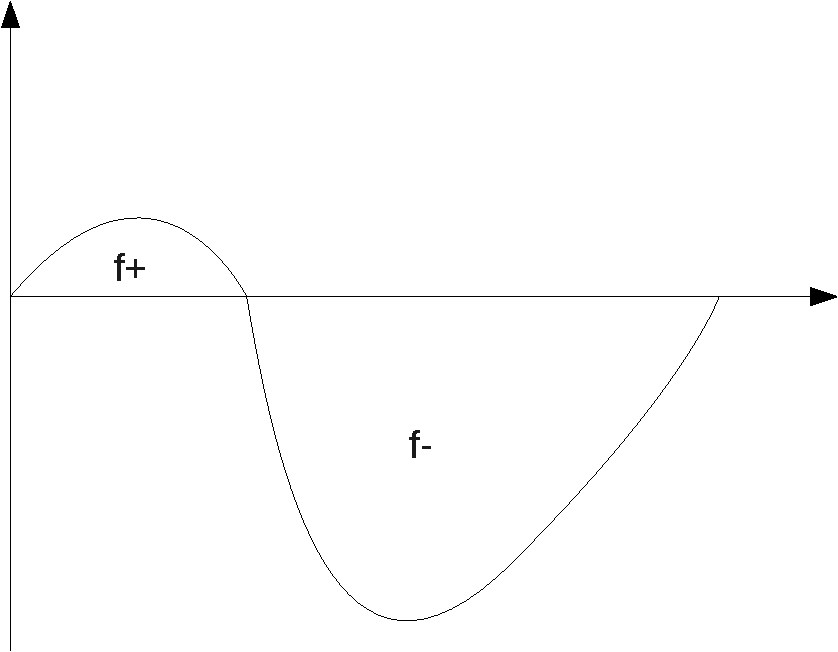
\includegraphics[scale=0.3]{images/fplus_fmoins.pdf}
\caption{Séparation partie positive/partie négative}\label{ch3:fig1}
\end{figure}
Pour toute application mesurable $f$, les applications $f^+,f^-$ sont
mesurables positives et admettent donc une intégrale. La définition de
l'intégrale de $f$ se fera à partir de celles de $f^+,f^-$.
\begin{mandatory}
\begin{defn}
Soit $f$ mesurable. On dira que $f$ est sommable si $f^+, f^-$ sont
sommables et on posera~:
\[
\int_E f d \mu = \int_E f^+ d \mu - \int_E f^- d \mu
\]
\end{defn}
\end{mandatory}
On notera que $|f|=f^++f^-$. Si $f$ est sommable, alors $|f|$ est sommable.
Réciproquement, si $|f|$ est sommable, alors $f^+,f^-$ sont nécessairement
sommables car:
\[
\int_E f^+ d \mu \leq \int_E |f| d \mu \quad \int_E f^- d \mu \leq \int_E |f|
\]
Il est donc équivalent, pour tester la sommabilité de $f$ de vérifier que $f$
est mesurable et que:
\[
\int_E |f| d \mu < +\infty
\]
C'est cette méthode qui est le plus souvent employée en pratique.
\begin{exercice}
Avec les notations et définitions de l'exercice \ref{ch3:ex1}, montrer que les
applications sommables sur $\left(\mathbb{N},\mathcal{P}(\mathbb{N})\right)$
sont les séries absolument convergentes.
\end{exercice}
On peut étendre la notion de sommabilité aux applications à valeurs complexes:
$f\colon E \to \mathbb{C}$ sera dite sommable si $\Re(f), \Im(f)$ sont
des applications sommables et on posera:
\[
\int_E f d\mu = \int_E \Re(f) d \mu + i \int_E
\Im(f) d \mu
\]
Une application mesurable $f \colon \mathbb{R} \to \mathbb{C}$ sera sommable si
et seulement $\Re(f), \Im(f)$ sont des applications mesurables et si:
\[
\int_E |f(x)| d \mu < +\infty
\]

\begin{mandatory}
\begin{prop}
Soient $f,g$ applications sommables et soit $\lambda \in \mathbb{R}$.
$\lambda f + g$ est sommable et~:
\[
\int_E \left( \lambda f + g\right) d \mu = \lambda \int_E f  d \mu + \int_E g d
\mu
\]
Si $f \leq g$~:
\[
\int_E f d \mu \leq \int_E g d \mu
\]
\end{prop}
\end{mandatory}
\begin{proof}
Supposons $\lambda > 0$. $(\lambda f )^+ =\lambda f^+$ et $(\lambda f + g)^+
\leq \lambda f^+ + g ^+$ d'où $(\lambda f + g )^+$ sommable. Un
raisonnement similaire sur les parties négatives montre que $(\lambda
f + g)^-$ est sommable, donc $\lambda f + g$ est
sommable. Par ailleurs, en décomposant $f$ et $g$ en parties positives
et négatives on a~
\[
\lambda f + g = \lambda f^+ + g^+ -(\lambda f^- +
g^-)
\]
d'où l'on obtient~:
\[
\int_E \lambda f + g d \mu = \lambda \int_E f d \mu + \int_E g d\mu
\]
Le cas $\lambda < 0$ se traite similairement en remarquant que
$(\lambda f)^+ = - \lambda f^-$.
Enfin, si $f \leq g$, $g-f \leq0$ est sommable d'intégrale $\int_E g-f
d \mu \geq 0 $, d'où $\int_E g d\mu - \int_E f d \mu \geq 0$.
\end{proof}
\begin{mandatory}
\begin{prop}
Soit $f$ une application sommable. On a~:
\[
\left |  \int_E f d \mu \right | \leq \int_E |f| d \mu
\]
\end{prop}
\end{mandatory}
\begin{proof}
$|f| = f^+ + f^-$ et~:
\[
\left | \int_E \left(f^+ - f^-\right) d \mu \right | \leq \int_E f^+ d \mu +
\int_E f^- d \mu = \int_E |f| d \mu
\]
\end{proof}
Le changement de variable et la relation de Chasles sont inchangées pour les
intégrales d'applications sommables.

\begin{defn}
Soit $(E, \mathcal{T}, \mu)$ un espace mesurable. Soit $\mathcal{P}$
une propriété définie sur $E$. On dira que $\mathcal{P}$ est vraie
$\mu$-presque partout (ou simplement presque partout si aucune
ambiguïté n'est possible sur la mesure) si~:
\[
\mu \left (
\{
x | \mathcal{P}(x) \mbox{ faux }
\}
\right ) = 0
\]
\end{defn}
\begin{mandatory}
\begin{prop}\label{ch2:upp}
Soient $f,g$ deux applications mesurables égales $\mu$-presque
partout. Si $g$ est sommable, alors $f$ est sommable et $\int_E f d
\mu = \int_E g d \mu$. 
\end{prop}
\end{mandatory}
\begin{proof}
Supposons dans un premier temps $f,g$ positives et $g$ sommable. 
Soit l'ensemble $A =
\{ x | f(x) \neq g(x) \}$.
La formule de Chasles donne ~:
\[
\int_E f\wedge n  d \mu = \int_A f\wedge n d \mu + \int_{A^c} f \wedge n d \mu
\]
Sur $A^c$, $f=g$ et donc:
\[
\int_{A^c} f \wedge n d \mu = \int_{A^c} g \wedge n d \mu
\]
D'où, comme $\mu(A)=0$ par hypothèse:
\[
\int_E f\wedge n  d \mu \leq \int_{A^c} g \wedge n d \mu + n \mu(A)\leq
\int_{E} g d \mu
\]
Par un passage à la limite, 
$\int_E f d\mu \leq \int_E g d \mu$, ce qui montre la sommabilité de $f$.
En échangeant les rôles de $f$ et $g$, on obtient finalement: $\int_E f d \mu =
\int_E g d \mu$. Si les applications ne sont pas positives mais sommables, on
applique le résultat précédent aux parties positives et négatives. 
\end{proof}
On utilise le plus souvent l'abbréviation $\mu\text{-pp}$ pour signifier qu'une
propriété est vraie $\mu$ presque partout.
